Fotovoltaika je technologie, která přímo přeměňuje sluneční záření na elektřinu.
K výrobě elektřiny není potřeba žádné palivo a elektrárny, proto se fotovoltaické elektrárny řadí mezi obnovitelné zdroje energie.


\section{Technický popis fotovoltaických elektráren}
% https://www.fotovia.cz/komponenty-fve

Při pořizování fotovoltaické elektrárny je k dobrému výběru dobré znát parametry jednotlivých částí, ze kterých se skládá.



\subsection{Veličiny}

\subsubsection{Watt} je jednotkou výkonu a rovná se vykonané práci za jendotku času.
Značíme symbolem \si{\watt}.

\subsubsection{Watt hodina} je jednotkou energie a rovná se práci stroje o výkonu jednoho wattu, který pracuje po dobu jedné hodiny.
Značíme ji symbolem \si{\watt\hour}. Při měření spotřeby elektřiny se nejčastěji se užívá v násobku kilowatt hodiny (\si{\kWh}).

\subsubsection{Killowatt--peak} je jednotkou špičkového výkonu fotovoltaické elektrárny. Tento výkon je při standardních testovacích podmínkách.
Značíme symbolem \si{\kW}p.


\subsection{Komponenty fotovoltaické elektrárny}
To, jaké komponenty se investor rozhodne koupit do svého fotovoltaického systému, může zásadně ovlivnit návratnost této investice.
Některé komponenty jsou pro elektrárnu nezbytné, jiné slouží k optimalizaci výkonu při různých podmínkách či specifickém využití.
Zde uvádím některé základní komponenty fotovoltaické elektrárny.

\subsubsection{Fotovoltaické panely}

jsou nezbytnou součástí každé fotovoltaické elektrárny.
Jejich hlavním úkolem je absorbovat sluneční záření a přeměnit ho na elektrickou energii.

\subsubsection{Baterie}

(nebo také akumulátory) slouží k ukládání přebytků energie, které nebyly spotřebovány.
Dělíme je na virtuální uložiště a fyzické uložiště.

\begin{itemize}
    \item \textbf{Virtuální uložiště} -- funguje na základě podepsání smlouvy s distributorem. Přebytky vyrobené energie se posílají do veřejné sítě, odkud se v případě potřeby mohou odčerpat.  Ve virtuální baterii můžete uložit tolik energie, kolik vám smluvně umožňuje distributor. Mají několik nevýhod:
    \begin{itemize}
        \item je to komerční produkt, který nenabízí všichni distributoři a nikde se negarantují stálé podmínky,
        \item platíte za využívání paušální poplatek,
        \item v případě výpadku elektřiny nemáte záložní zdroj energie.
    \end{itemize}
    \item \textbf{Fyzické bateriové uložiště} -- je zařízení, které je uložené v domě. Vyrobená energie se do baterií ukládá a v případě potřeby se z nich odebírá. Nevýhodou fyzické baterie je její kapacita.
\end{itemize}


% \subsubsection{Virtuální uložiště}
% funguje na základě podepsání smlouvy s distributorem. Přebytky vyrobené energie se posílají do veřejné sítě, odkud se v případě potřeby mohou odčerpat.
% Virtuální úložiště nejsou plnou náhradou fyzických baterií. Mají několik nevýhod:

% \begin{itemize}
%     \item je to komerční produkt, který nenabízí všichni distributoři a nikde se negarantují stálé podmínky,
%     \item platíte za využívání paušální poplatek,
%     \item v případě výpadku elektřiny nemáte záložní zdroj energie. 
% \end{itemize}

% \subsubsection{Fyzické bateriové uložiště} je zařízení, které je uložené v domě. Vyrobená energie se do baterií ukládá a v případě potřeby se z nich odebírá.
% Nevýhodou fyzické baterie je její kapacita. Ve virtuální baterii můžete uložit tolik energie, kolik vám smluvně umožňuje distributor.


\subsubsection{Invertor}

(nebo také měnič či střídač) je podobně jako fotovoltaické panely
nezbytnou součástí každé fotovoltaické elektrárny.
Jeho hlavní funkcí je přeměna stejnosměrného proudu na proud střídavý.
Inverotr rozděluje vyrobenou energii do tří fází. To kolik dávkuje do jednotlivých fází záleží na typu invertoru.

\begin{itemize}
    \item Symetrikcý invertor -- levnější typ, dávkuje elektřinu rovnoměrně do všech tří fází.
    \item Asymetrický invertor -- dražší typ, při dávkování zohledňuje spotřebu na všech fázích.
\end{itemize}

Pokud by tedy například fotovoltaika vyrobila 6 \si{\kWh} elektřiny a spotřeba by na jednotlivých fázích vypdala následovně:

\begin{itemize}
    \item Fáze 1: 3 \si{\kWh}
    \item Fáze 2: 2 \si{\kWh}
    \item Fáze 3: 0.5 \si{\kWh}
\end{itemize}

Symetrický invertor rozdělí elektřinu rovnoměrně (2 \si{\kWh} na každou fázi), takže na fázi 2 a 3 vznikne přebytek, který se pošle do sítě a na fázi 1 energie chybí, tzn. musí se dobrat ze sítě.
Asymetrický invertor elektřinu rozdělí tak, že nebude nutné ze sítě nic dobírat, ani do ní nic posílat.  

\subsubsection{Optimizér}
je zařízení, které se připojuje k jednotlivým fotovoltaickým panelům. Výkon elektrárny se odvíjí od výkony nejméně vákoného článku.
V případě že je snížen výkon jednoho panelu, optimizér zajistí přemostění tohoto panelu.


\subsection{Druhy fotovoltaických systémů}
% https://www.fotovia.cz/blog/typy-fotovoltaickych-elektraren

Rozdílem mezi jednotlivými druhy fotovoltaických systémů je jejich napojení do veřejné elektrické sítě a integrace akumulátorů.
Podle těchto kritérií je lze rozdělit do tří základních kategorií:

\begin{itemize}
    \item ostrovní
    \item standardní
    \item hybridní
\end{itemize}

\subsubsection{Ostrovní elektrárna}

(tzv. off-grid) je samostatný systém, který není připojen k elektrické síti.
Klíčovou částí toho systému je baterie (akumulátor), která slouží k ukládání přebytků energie.
Jsou užitečné v oblastech, kde připojení k elektrické síti není možné.

\begin{multicols}{2}
    \textbf{Výhody:}
    \begin{itemize}[leftmargin=*]
        \item nezávislost na dodavatelích elektřiny,
        \item pokud dojde k výpadku elektřiny, ostrovní elektrárna bude sloužit jako záložní zdroj,
    \end{itemize}
    
    \columnbreak
    
    \textbf{Nevýhody:}
    \begin{itemize}[leftmargin=*]
        \item počáteční náklady mohou být vyšší, kvůli potřebě akumulátorů,
        \item baterie vyžadují pravidelnou údržbu.
    \end{itemize}
\end{multicols}

\begin{figure}[h]
    \centering
    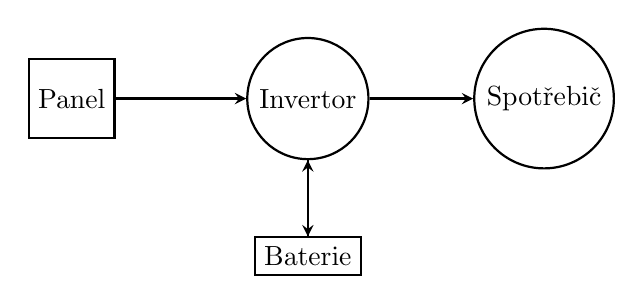
\begin{tikzpicture}[>=stealth,thick]
        % Nodes
        \node[draw, minimum height=1cm] (panel) at (0,0) {Panel};
        \node[draw, circle] (inverter) at (3,0) {Invertor};
        \node[draw] (baterie) at (3,-2) {Baterie};
        \node[draw, circle] (odb) at (6,0) {Spotřebič};
        % Arrows
        \draw[->] (panel) -- (inverter);
        \draw[->] (inverter) -- (baterie);
        \draw[->] (baterie) -- (inverter);
        \draw[->] (inverter) -- (odb);

    \end{tikzpicture}
    \caption{Schéma off-grid fotovoltaické elektrárny}
    \label{fig:offgrid_schema}
\end{figure}

\subsubsection{Standardní elektrárna}

Standardní (tzv. on-grid) fotovoltaická elektrárna je připojena k elektrické síti.
Veškerou přebytečnou energii lze prodat dodavateli elektřiny a v případě potřeby ji lze i odebírat.

\begin{multicols}{2}
    \textbf{Výhody:}
    \begin{itemize}[leftmargin=*]
        \item možnost prodeje přebytků elektřiny,
        \item dlouhá životnost, malá potřeba údržby.
    \end{itemize}
    
    \columnbreak
    
    \textbf{Nevýhody:}
    \begin{itemize}[leftmargin=*]
        \item závislost na síti,
        \item závislost na slunečním záření.
    \end{itemize}
\end{multicols}


\begin{figure}[H]
    \centering
    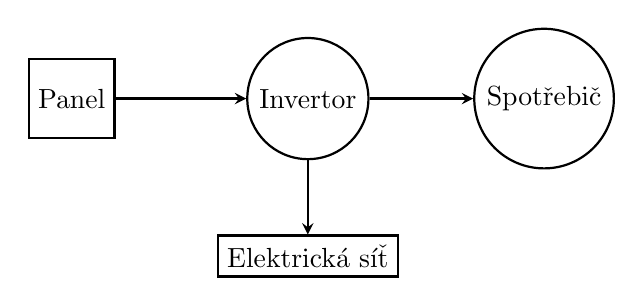
\begin{tikzpicture}[>=stealth,thick]
        % Nodes
        \node[draw, minimum height=1cm] (panel) at (0,0) {Panel};
        \node[draw, circle] (inverter) at (3,0) {Invertor};
        \node[draw, circle] (odb) at (6,0) {Spotřebič};
        \node[draw, minimum width=2cm] (sita) at (3,-2) {Elektrická síť};
        % Arrows
        \draw[->] (panel) -- (inverter);
        \draw[->] (inverter) -- (odb);
        \draw[->] (inverter) -- (sita);

    \end{tikzpicture}
    \caption{Schéma on-grid fotovoltaické elektrárny}
    \label{fig:ongrid_schema}
    \end{figure}


\subsubsection{Hybridní elektrárna}

kombinuje výhody ostrovních a standardních systémů.
Jsou připojeny k elektrické síti, ale zároveň mají akumulátory, které slouží jako záložní zdroj energie.

\begin{multicols}{2}
    \textbf{Výhody:}
    \begin{itemize}[leftmargin=*]
        \item uložení přebytků energie,
        \item větší energetická nezávislost.
    \end{itemize}
    
    \columnbreak
    
    \textbf{Nevýhody:}
    \begin{itemize}[leftmargin=*]
        \item vysoké počáteční náklady,
        \item baterie vyžadují pravidelnou údržbu.
    \end{itemize}

\end{multicols}

\begin{figure}[h]
    \centering
    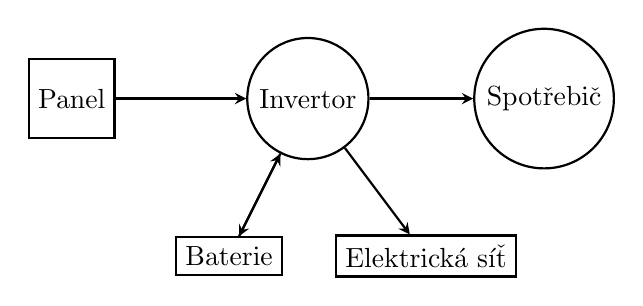
\begin{tikzpicture}[>=stealth,thick]
        % Nodes
        \node[draw, minimum height=1cm] (panel) at (0,0) {Panel};
        \node[draw, circle] (inverter) at (3,0) {Invertor};
        \node[draw] (baterie) at (2,-2) {Baterie};
        \node[draw, circle] (odb) at (6,0) {Spotřebič};
        \node[draw, minimum width=2cm] (sita) at (4.5,-2) {Elektrická síť};
        % Arrows
        \draw[->] (panel) -- (inverter);
        \draw[->] (inverter) -- (baterie);
        \draw[->] (baterie) -- (inverter);
        \draw[->] (inverter) -- (odb);
        \draw[->] (inverter) -- (sita);

    \end{tikzpicture}
    \caption{Schéma hybridní fotovoltaické elektrárny}
    \label{fig:hybrid_schema}
\end{figure}


\section{Jak fotovoltaika šetří peníze}
% https://oze.tzb-info.cz/fotovoltaika/24229-stroj-na-penize-fotovoltaika-pri-vysokych-cenach-elektriny-usetri-desetitisice-korun-rocne
Fotovoltaické elektrárny představují významný způsob, jak snižovat náklady na elektřinu v domácnostech.
V domácnosti přispívá fotovoltaika k úspoře peněz dvěma hlavními způsoby.

% \begin{itemize}
%     \item Vyrobená elektřina, která se spotřebuje na místě, se nemusí nakoupit ze sítě.
%     \item Přebytek elektřiny se prodá dodavateli do sítě
% \end{itemize}
\subsection{Spotřeba vyrobené elektřiny}

Vyrobená elektřina, která se spotřebuje na místě, se nemusí nakoupit ze sítě.
Pro tuto úsporu jsou důležité dva faktory:

\begin{itemize}
    \item \textbf{Kolik elektřiny fotovoltaika vyrobí.} V ČR je horní limit pro výkon domácí elektrárny 10 \si{\kW}p. Pokud pro hrubý odhad výroby použijeme jednoduchý přepočet, kdy 1 instalovaný \si{\kW}p vyrobí za rok 1 MWh, zjistíme, že v ČR lze ročně ušetřit maximálně 10 MWh. Na vyšší výkon je potřeba licence nebo provoz v ostrovním režimu.
    \item \textbf{Kolik elektřiny domácnost spotřebuje.} Fotovoltaika vyrábí nejvíce elektřiny vyrábí přes den a v létě. Největší spotřeba domácnosti je ale v zimě a večer. Spotřeba domácnosti
\end{itemize}

% 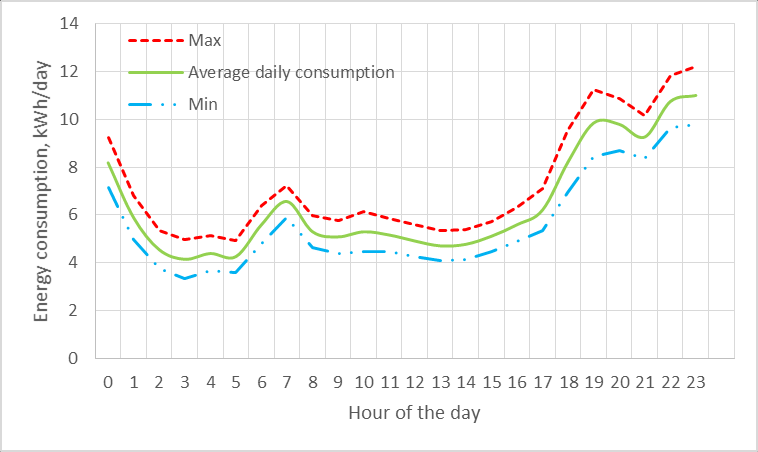
\includegraphics[width=\textwidth]{static/average-daily-consumption.png}
\begin{figure}
    % https://www.researchgate.net/publication/326358349_Load_Profile_of_Typical_Residential_Buildings_in_Bulgaria
    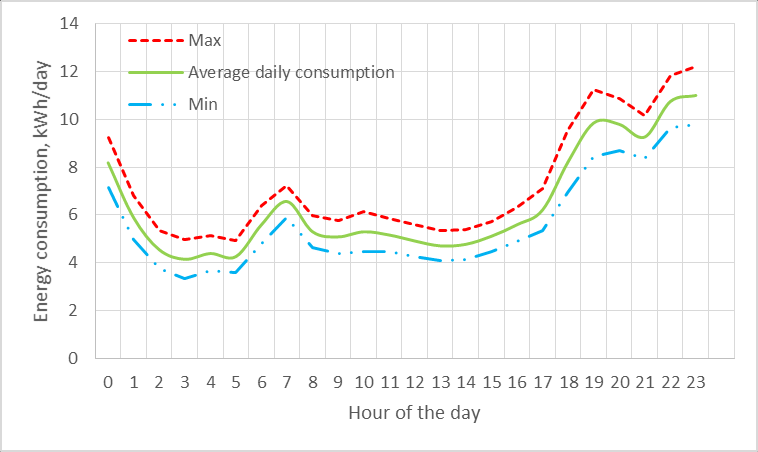
\includegraphics[width=\textwidth]{static/average-daily-consumption.png}
    \caption{Denní spotřeba elektřiny v domácnosti během všedního dne.} % Zdroj: \cite{bulgaria}
    \label{fig:average_daily_consumption}
\end{figure}

\subsection{Prodej přebytků elektřiny}
